\documentclass{standalone}
\usepackage{tikz}
\begin{document}
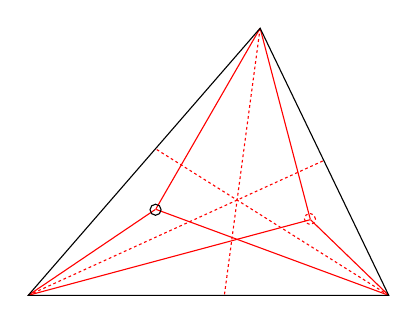
\begin{tikzpicture}[x=1pt,y=1pt]
\draw[red, dash pattern=on 1pt] (114.03,-76.40) -- (101.11,-172.92);
\draw[red, dash pattern=on 1pt] (30.24,-172.92) -- (137.05,-124.20);
\draw[red, dash pattern=on 1pt] (160.50,-172.92) -- (76.22,-119.95);
\draw[red] (114.03,-76.40) -- (76.39,-141.66);
\draw[red] (30.24,-172.92) -- (76.23,-141.86);
\draw[red] (160.50,-172.92) -- (76.48,-141.88);
\draw[red] (114.03,-76.40) -- (132.17,-145.46);
\draw[red] (160.50,-172.92) -- (132.22,-145.58);
\draw[red] (30.24,-172.92) -- (132.07,-145.61);
\draw (76.25,-141.99) circle (2.00);
\draw[red, dash pattern=on 1pt] (132.05,-145.31) circle (2.00);
\draw (160.50,-172.92) -- (114.04,-76.40) -- (30.24,-172.92) -- cycle;
\end{tikzpicture}
\end{document}
